% Practice Test 03 — Florida Edition
% Questions: 30 (21 MC + 9 SA)
% Generated by scripts/generate_practice_tests.py

\begin{practiceQuestion}{1-3-q29}{gsa}
\begin{questionText}
The graph shows a proportional relationship. Use the labeled point to find $k$, then determine $y$ when $x = 12$.

\begin{center}
\begin{tikzpicture}[scale=0.6]
  \draw[step=1,gray!20,thin] (0,0) grid (8,8);
  \draw[thick,->] (0,0) -- (8.5,0) node[right]{\small $x$};
  \draw[thick,->] (0,0) -- (0,8.5) node[above]{\small $y$};
  \foreach \x in {2,4,6,8} \draw (\x,0.07) -- (\x,-0.07) node[below]{\tiny \x};
  \foreach \y in {2,4,6,8} \draw (0.07,\y) -- (-0.07,\y) node[left]{\tiny \y};
  \draw[thick,funBlue] (0,0) -- (8,6);
  \fill[funBlue] (0,0) circle (2.5pt);
  \fill[funBlue] (4,3) circle (2.5pt) node[above left]{\small $(4, 3)$};
\end{tikzpicture}
\end{center}
\end{questionText}
\correctAnswer{$k = 0.75$; when $x = 12$, $y = 9$}
\explanation{$k = \frac{3}{4} = 0.75$. Then $y = 0.75 \times 12 = 9$.}
\end{practiceQuestion}

\begin{practiceQuestion}{1-6-q12}{mc}
\begin{questionText}
Store A sells $3$ notebooks for $\$7.50$. Store B sells $5$ notebooks for $\$11.25$. Which store offers the better deal?
\end{questionText}
\choiceA{Store A at $\$2.50$ each}
\choiceB{Store B at $\$2.25$ each}
\choiceC{Store A at $\$2.25$ each}
\choiceD{They cost the same}
\correctAnswer{B}
\explanation{Store A: $7.50 \div 3 = \$2.50$ each. Store B: $11.25 \div 5 = \$2.25$ each. Store B is cheaper.}
\end{practiceQuestion}

\begin{practiceQuestion}{2-1-q11}{mc}
\begin{questionText}
A baker made $120$ cupcakes and sold $90$ of them. What percent of the cupcakes were sold?
\end{questionText}
\choiceA{$60\%$}
\choiceB{$70\%$}
\choiceC{$75\%$}
\choiceD{$80\%$}
\correctAnswer{C}
\explanation{Divide: $90 \div 120 = 0.75 = 75\%$.}
\end{practiceQuestion}

\begin{practiceQuestion}{2-2-q25}{sa}
\begin{questionText}
A farmer harvested $420$ apples. He sold $315$ of them. What percent did he sell?
\end{questionText}
\correctAnswer{$75\%$}
\explanation{$\frac{315}{420} = \frac{p}{100}$. Cross-multiply: $420p = 31{,}500$. Divide: $p = 75\%$.}
\end{practiceQuestion}

\begin{practiceQuestion}{2-6-q26}{gmc}
\begin{questionText}
The graph below shows the total amount in a simple interest savings account over time. What is the annual interest rate?

\begin{center}
\begin{tikzpicture}[scale=0.7]
  \draw[thick,->] (0,0) -- (6,0) node[right]{\small Years};
  \draw[thick,->] (0,0) -- (0,6) node[above]{\small Total (\$)};
  \draw[gray!20,thin] (0,0) grid[step=1] (5,5);
  \foreach \x in {0,...,5} {
    \node[below,font=\small] at (\x,0) {$\x$};
  }
  \foreach \y/\lab in {1/200,2/400,3/600,4/800,5/1000} {
    \draw (-0.1,\y) -- (0.1,\y) node[left,font=\small,xshift=-2pt] {\lab};
  }
  % Points: P = 800, r = 5%, so total = 800 + 40t
  % t=0: 800, t=1: 840, t=2: 880, t=3: 920, t=4: 960, t=5: 1000
  \filldraw[funBlue] (0,4) circle (3pt);
  \filldraw[funBlue] (1,4.2) circle (3pt);
  \filldraw[funBlue] (2,4.4) circle (3pt);
  \filldraw[funBlue] (3,4.6) circle (3pt);
  \filldraw[funBlue] (4,4.8) circle (3pt);
  \filldraw[funBlue] (5,5) circle (3pt);
  \draw[thick,funBlue] (0,4) -- (1,4.2) -- (2,4.4) -- (3,4.6) -- (4,4.8) -- (5,5);
  \node[right,font=\small] at (0.1,4) {$\$800$};
  \node[right,font=\small] at (5.1,5) {$\$1{,}000$};
\end{tikzpicture}
\end{center}
\end{questionText}
\choiceA{$4\%$}
\choiceB{$5\%$}
\choiceC{$8\%$}
\choiceD{$10\%$}
\correctAnswer{B}
\explanation{Principal: $\$800$. After $5$ years: $\$1{,}000$. Interest: $1{,}000 - 800 = \$200$. Rate: $200 = 800 \times r \times 5$ → $r = 200 \div 4{,}000 = 0.05 = 5\%$.}
\end{practiceQuestion}

\begin{practiceQuestion}{2-7-q18}{mc}
\begin{questionText}
A package was estimated to weigh $10$ kg, but it actually weighs $12$ kg. A second package was estimated to weigh $50$ kg, but it actually weighs $52$ kg. Which estimate has the smaller percent error?
\end{questionText}
\choiceA{The first package}
\choiceB{The second package}
\choiceC{They have the same percent error}
\choiceD{Cannot be determined}
\correctAnswer{B}
\explanation{First: $\frac{2}{12} \times 100 \approx 16.7\%$. Second: $\frac{2}{52} \times 100 \approx 3.8\%$. The second has a smaller percent error.}
\end{practiceQuestion}

\begin{practiceQuestion}{3-2-q26}{gmc}
\begin{questionText}
The number line shows a move starting at $-2$. What addition does the arrow represent?

\begin{center}
\begin{tikzpicture}
  \draw[thick,->] (-6.5,0) -- (6.5,0);
  \foreach \x in {-6,...,6} \draw (\x,0.1) -- (\x,-0.1) node[below] {$\x$};
  \draw[thick,->,funBlue] (-2,0.4) -- (3,0.4);
  \node[above,funBlue] at (0.5,0.4) {$+5$};
\end{tikzpicture}
\end{center}
\end{questionText}
\choiceA{$(-2) + 5 = 3$}
\choiceB{$(-2) + (-5) = -7$}
\choiceC{$3 + (-5) = -2$}
\choiceD{$5 + (-2) = 7$}
\correctAnswer{A}
\explanation{The arrow starts at $-2$ and moves $5$ units to the right, landing at $3$. This shows $(-2) + 5 = 3$.}
\end{practiceQuestion}

\begin{practiceQuestion}{3-3-q19}{sa}
\begin{questionText}
What is $(-14) - 6$?
\end{questionText}
\correctAnswer{$-20$}
\explanation{$(-14) - 6 = (-14) + (-6) = -20$. Same signs: add and keep negative.}
\end{practiceQuestion}

\begin{practiceQuestion}{4-4-q12}{mc}
\begin{questionText}
Factor $20n - 30$.
\end{questionText}
\choiceA{$5(4n - 6)$}
\choiceB{$10(2n - 3)$}
\choiceC{$2(10n - 15)$}
\choiceD{$20(n - 30)$}
\correctAnswer{B}
\explanation{GCF of $20$ and $30$ is $10$. Factor: $20n \div 10 = 2n$ and $-30 \div 10 = -3$. Result: $10(2n - 3)$.}
\end{practiceQuestion}

\begin{practiceQuestion}{4-5-q11}{mc}
\begin{questionText}
Simplify $(\frac{1}{2}x + 3) + (\frac{3}{2}x - 5)$.


\fractionBar{1}{2}
\end{questionText}
\choiceA{$x - 2$}
\choiceB{$2x - 2$}
\choiceC{$2x + 8$}
\choiceD{$x + 8$}
\correctAnswer{B}
\explanation{Combine: $(\frac{1}{2}x + \frac{3}{2}x) + (3 - 5) = \frac{4}{2}x - 2 = 2x - 2$.}
\end{practiceQuestion}

\begin{practiceQuestion}{5-3-q16}{mc}
\begin{questionText}
Solve $8(x + 1) = 48$.
\end{questionText}
\choiceA{$x = 5$}
\choiceB{$x = 6$}
\choiceC{$x = 7$}
\choiceD{$x = \dfrac{47}{8}$}
\correctAnswer{A}
\explanation{Divide by $8$: $x + 1 = 6$. Subtract $1$: $x = 5$. Check: $8(5 + 1) = 8(6) = 48$ \checkmark.}
\end{practiceQuestion}

\begin{practiceQuestion}{5-4-q13}{mc}
\begin{questionText}
A shirt is on sale for $\dfrac{2}{3}$ of its original price. After using a $\$5$ coupon, you pay $\$15$. What equation finds the original price $p$?
\end{questionText}
\choiceA{$\dfrac{2}{3}p + 5 = 15$}
\choiceB{$p - \dfrac{2}{3} - 5 = 15$}
\choiceC{$\dfrac{2}{3}p - 5 = 15$}
\choiceD{$\dfrac{2}{3}(p - 5) = 15$}
\correctAnswer{C}
\explanation{Sale price is $\frac{2}{3}p$. After the $\$5$ coupon: $\frac{2}{3}p - 5 = 15$.}
\end{practiceQuestion}

\begin{practiceQuestion}{5-5-q02}{mc}
\begin{questionText}
Solve $-3n + 6 \leq 0$.
\end{questionText}
\choiceA{$n \leq 2$}
\choiceB{$n \leq -2$}
\choiceC{$n \geq 2$}
\choiceD{$n \geq -2$}
\correctAnswer{C}
\explanation{Subtract $6$: $-3n \leq -6$. Divide by $-3$ and flip the sign: $n \geq 2$.}
\end{practiceQuestion}

\begin{practiceQuestion}{5-6-q05}{mc}
\begin{questionText}
Which inequality is shown by a closed circle at $7$ with shading to the left?
\end{questionText}
\choiceA{$x > 7$}
\choiceB{$x < 7$}
\choiceC{$x \geq 7$}
\choiceD{$x \leq 7$}
\correctAnswer{D}
\explanation{Closed circle means the endpoint is included, shading left means less than or equal to: $x \leq 7$.}
\end{practiceQuestion}

\begin{practiceQuestion}{6-2-q27}{gmc}
\begin{questionText}
The two rectangles below represent the same room drawn at two different scales. The original uses $1$ cm $= 6$ m. What scale does the new drawing use?

\begin{center}
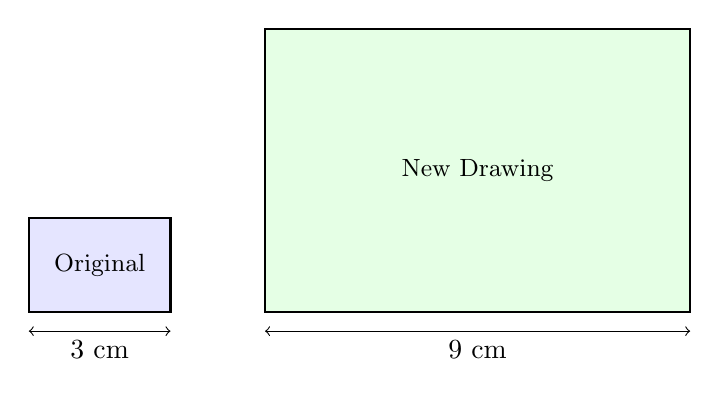
\begin{tikzpicture}[scale=0.6]
  % Original
  \draw[thick,fill=blue!10] (0,0) rectangle (3,2);
  \node at (1.5,1) {\small Original};
  \draw[<->] (0,-0.4) -- (3,-0.4);
  \node[below] at (1.5,-0.4) {$3$ cm};
  % New
  \draw[thick,fill=green!10] (5,0) rectangle (14,6);
  \node at (9.5,3) {\small New Drawing};
  \draw[<->] (5,-0.4) -- (14,-0.4);
  \node[below] at (9.5,-0.4) {$9$ cm};
\end{tikzpicture}
\end{center}
\end{questionText}
\choiceA{$1$ cm $= 2$ m}
\choiceB{$1$ cm $= 3$ m}
\choiceC{$1$ cm $= 6$ m}
\choiceD{$1$ cm $= 18$ m}
\correctAnswer{A}
\explanation{Scale ratio: $9 \div 3 = 3$. The new drawing is $3$ times bigger. Actual length: $3 \times 6 = 18$ m. New scale: $18 \div 9 = 2$ m per cm.}
\end{practiceQuestion}

\begin{practiceQuestion}{6-4-q20}{sa}
\begin{questionText}
Can a triangle have sides $8$, $8$, and $16$? Explain.
\end{questionText}
\correctAnswer{No}
\explanation{$8 + 8 = 16$, which is not greater than $16$. The triangle inequality requires the sum to be strictly greater.}
\end{practiceQuestion}

\begin{practiceQuestion}{6-5-q25}{sa}
\begin{questionText}
A square pyramid has a base edge of $8$ cm. It is sliced parallel to the base halfway up. Is the cross-section larger, smaller, or the same size as the base?
\end{questionText}
\correctAnswer{Smaller than the base}
\explanation{A horizontal cut parallel to the base of a pyramid produces a similar shape that is smaller than the base. Halfway up, the cross-section is a $4$ cm square (half the edge length).}
\end{practiceQuestion}

\begin{practiceQuestion}{6-6-q01}{mc}
\begin{questionText}
Two angles are supplementary. One angle is $115°$. What is the other angle?
\end{questionText}
\choiceA{$25°$}
\choiceB{$55°$}
\choiceC{$65°$}
\choiceD{$75°$}
\correctAnswer{C}
\explanation{Supplementary angles sum to $180°$. $180° - 115° = 65°$.}
\end{practiceQuestion}

\begin{practiceQuestion}{7-1-q05}{mc}
\begin{questionText}
A circle has a diameter of $9$ feet. What is its radius?
\end{questionText}
\choiceA{$18$ feet}
\choiceB{$9$ feet}
\choiceC{$4.5$ feet}
\choiceD{$3$ feet}
\correctAnswer{C}
\explanation{The radius is half the diameter: $r = 9 \div 2 = 4.5$ feet.}
\end{practiceQuestion}

\begin{practiceQuestion}{7-5-q06}{mc}
\begin{questionText}
A gift box is $8$ cm by $5$ cm by $3$ cm. How much wrapping paper is needed to cover the entire box?
\end{questionText}
\choiceA{$79$ cm$^2$}
\choiceB{$120$ cm$^2$}
\choiceC{$158$ cm$^2$}
\choiceD{$316$ cm$^2$}
\correctAnswer{C}
\explanation{$SA = 2(8 \times 5) + 2(8 \times 3) + 2(5 \times 3) = 80 + 48 + 30 = 158$ cm$^2$.}
\end{practiceQuestion}

\begin{practiceQuestion}{7-6-q30}{gsa}
\begin{questionText}
A rectangular prism-shaped fish tank is shown below. If water fills the tank to $\frac{3}{4}$ of its height, what is the volume of water in the tank?

\begin{center}
\begin{tikzpicture}[scale=0.35]
  % Tank outline
  \draw[thick,funBlue] (0,0) rectangle (10,8);
  \draw[thick,funBlue] (10,0) -- (14,3) -- (14,11) -- (10,8);
  \draw[thick,funBlue] (0,8) -- (4,11) -- (14,11);
  % Water level at 3/4
  \fill[cyan!30] (0,0) rectangle (10,6);
  \fill[cyan!20] (10,0) -- (14,3) -- (14,9) -- (10,6) -- cycle;
  \draw[dashed,funRed] (0,6) -- (10,6) -- (14,9);
  \node[left,funRed] at (0,6) {water};
  % Labels
  \draw[thick,funRed,<->] (0,-0.8) -- (10,-0.8);
  \node[below,funRed] at (5,-0.8) {$20$ cm};
  \draw[thick,funRed,<->] (-1,0) -- (-1,8);
  \node[left,funRed] at (-1,4) {$16$ cm};
  \draw[thick,funRed,<->] (14.5,3) -- (14.5,11);
  \node[right,funRed] at (14.5,7) {$16$ cm};
  \node[below right,funRed] at (12,1.5) {$10$ cm};
\end{tikzpicture}
\end{center}
\end{questionText}
\correctAnswer{$2{,}400$ cm$^3$}
\explanation{Full tank volume: $20 \times 10 \times 16 = 3{,}200$ cm$^3$. Water at $\frac{3}{4}$ height: $20 \times 10 \times 12 = 2{,}400$ cm$^3$.}
\end{practiceQuestion}

\begin{practiceQuestion}{7-7-q14}{mc}
\begin{questionText}
A cylindrical container has a volume of $628$ cm$^3$ and a height of $8$ cm. What is the radius? Use $\pi \approx 3.14$.
\end{questionText}
\choiceA{$3$ cm}
\choiceB{$4$ cm}
\choiceC{$5$ cm}
\choiceD{$6$ cm}
\correctAnswer{C}
\explanation{$628 = 3.14 \times r^2 \times 8 = 25.12 \, r^2$. $r^2 = 628 \div 25.12 = 25$. $r = 5$ cm.}
\end{practiceQuestion}

\begin{practiceQuestion}{8-1-q02}{mc}
\begin{questionText}
A researcher wants to know the average height of seventh graders in a state. She measures the heights of $100$ seventh graders from different schools. What is the sample?
\end{questionText}
\choiceA{All seventh graders in the state}
\choiceB{All students in the schools she visited}
\choiceC{The $100$ seventh graders she measured}
\choiceD{The tallest seventh graders}
\correctAnswer{C}
\explanation{The sample is the smaller group chosen from the population — the $100$ students measured.}
\end{practiceQuestion}

\begin{practiceQuestion}{8-3-q24}{sa}
\begin{questionText}
Class A: median $90$, IQR $6$. Class B: median $83$, IQR $14$. Which class is more consistent?
\end{questionText}
\correctAnswer{Class A}
\explanation{Class A has a smaller IQR ($6$ vs.\ $14$), meaning the middle $50\%$ of scores are more tightly clustered.}
\end{practiceQuestion}

\begin{practiceQuestion}{8-4-q19}{sa}
\begin{questionText}
Data: $30, 35, 40, 45, 50$. Find the mean and range.
\end{questionText}
\correctAnswer{Mean $= 40$; Range $= 20$}
\explanation{Mean: $\frac{30+35+40+45+50}{5} = \frac{200}{5} = 40$. Range: $50 - 30 = 20$.}
\end{practiceQuestion}

\begin{practiceQuestion}{8-5-q04}{mc}
\begin{questionText}
Data: $12, 15, 21, 23, 27, 30, 35$. In a stem-and-leaf plot, what are the stems?
\end{questionText}
\choiceA{$1, 2, 3$}
\choiceB{$2, 5, 1, 3, 7, 0, 5$}
\choiceC{$12, 15, 21, 23, 27, 30, 35$}
\choiceD{$10, 20, 30$}
\correctAnswer{A}
\explanation{The stems are the tens digits: $1$ (for $12, 15$), $2$ (for $21, 23, 27$), $3$ (for $30, 35$).}
\end{practiceQuestion}

\begin{practiceQuestion}{8-6-q13}{mc}
\begin{questionText}
Which is NOT a good use of a circle graph?
\end{questionText}
\choiceA{Showing the breakdown of a budget}
\choiceB{Showing parts of a whole survey result}
\choiceC{Comparing temperatures over time}
\choiceD{Showing how students spend their time}
\correctAnswer{C}
\explanation{Circle graphs show parts of a whole. For data that changes over time, a line graph is more appropriate.}
\end{practiceQuestion}

\begin{practiceQuestion}{9-4-q27}{gmc}
\begin{questionText}
The table shows a probability model for a spinner. The spinner is spun $100$ times and the results are shown. Does the observed data support the model?

\begin{center}
\begin{tabular}{|c|c|c|}
\hline
\textbf{Color} & \textbf{Model $P$} & \textbf{Observed Frequency} \\
\hline
Red & $0.40$ & $38$ \\
\hline
Blue & $0.35$ & $36$ \\
\hline
Yellow & $0.25$ & $26$ \\
\hline
\end{tabular}
\end{center}
\end{questionText}
\choiceA{No, the data is very different from the model}
\choiceB{Yes, the observed frequencies are close to the predicted values}
\choiceC{No, because Red appeared fewer times than predicted}
\choiceD{The model cannot be checked with only $100$ spins}
\correctAnswer{B}
\explanation{Predicted: Red $= 40$, Blue $= 35$, Yellow $= 25$. Observed: $38$, $36$, $26$. These are close, supporting the model.}
\end{practiceQuestion}

\begin{practiceQuestion}{9-6-q01}{mc}
\begin{questionText}
What is the probability of flipping two coins and getting heads on both?
\end{questionText}
\choiceA{$\frac{1}{2}$}
\choiceB{$\frac{1}{3}$}
\choiceC{$\frac{1}{4}$}
\choiceD{$\frac{3}{4}$}
\correctAnswer{C}
\explanation{Sample space: HH, HT, TH, TT ($4$ outcomes). Only HH is heads-heads. $P = \frac{1}{4}$.}
\end{practiceQuestion}

\begin{practiceQuestion}{9-7-q20}{sa}
\begin{questionText}
You roll a die $90$ times to simulate a $\frac{1}{6}$ probability event. How many times do you expect the event to occur?
\end{questionText}
\correctAnswer{$15$}
\explanation{$90 \times \frac{1}{6} = 15$.}
\end{practiceQuestion}
